\section{Background and Motivation}
\label{background}
This section first gives a brief background of congestion 
control in the datacenter. Then the motivation for moving congestion
control into the vSwitch is presented. Finally,~\acdc{} is contrasted from a class of related bandwidth
allocation schemes.

\subsection{Datacenter Transport}
\label{ss:dct}
Today's datacenters host applications such as search,
advertising, analytics and retail that require high bandwidth and low latency.
%Large tail latencies often violate the tight timing constraints required by SLAs at scale, and
%have been shown to impact customer experience, result in
%revenue loss~\cite{dctcp,dean2013tail}, and degrade application performance~\cite{jang2015silo,qjump}.
%Tail latencies are often caused by network congestion.
%The latency of traversing a single switch, NIC and OS network stack is 10--30$\mu$s,
%2.5--32$\mu$s and 15$\mu$s respectively, but a congested port
%on a network switch can consume significant shared memory, causing orders-of-magnitude
%higer latency~\cite{rumble2011s}.
Network congestion, caused by imperfect load balancing~\cite{hedera},
network upgrades or failures, can adversely impact these services. Unfortunately, congestion is
not rare in datacenters. For example, recently Google reported 
congestion-based drops were observed when network utilization approached 25\%~\cite{singh2015jupiter}.
Other studies have shown high variance and substantial increase in the 99.9$^{th}$ percentile latency
for round-trip times in today's datacenters~\cite{wang2010impact,mogul2015inferring}. 
Large tail latencies impact customer experience, result in
revenue loss~\cite{dctcp,dean2013tail}, and degrade application performance~\cite{jang2015silo,qjump}.
Therefore, significant motivation exists to reduce congestion in datacenter fabrics.

%Studies have shown that while CUBIC can achieve
%high bandwidth, it does so at the cost of aggressively filling up the switch buffers in the network.
TCP's congestion control algorithm is
known to significantly impact network performance.
As a result, datacenter TCP performance has been widely
studied and many new protocols have been proposed~\cite{dctcp, stephens2014practical, wu2010ictcp,
mittal2015timely, jose2015high}. Specifically, DCTCP~\cite{dctcp} adjusts a TCP sender's rate based on the fraction of packets experiencing congestion. In DCTCP,
the switches are configured to mark packets with an ECN bit when their queue lengths exceed a threshold. By proportionally
adjusting the rate of the sender based on the fraction of ECN bits received, DCTCP can keep queue lengths low, 
maintain high throughput, and increase fairness and stability over traditional schemes~\cite{dctcp,judd2015nsdi}.
\crs{For these reasons, we implement DCTCP as the vSwitch congestion control algorithm in~\acdc{}.}

\subsection{Benefits of~\acdc{}}
%Rather than proposing a new datacenter congestion control algorithm, this work investigates
%if congestion control can be moved to the vSwitch.
Allowing administrators to enforce an optimized congestion control without
changing the VM is the first major benefit of our scheme.
This is an important criteria in untrusted public cloud environments or simply in cases where servers cannot be updated
due to a dependence on a specific OS or library.~\cite{judd2015nsdi}


\begin{figure}[!t]
        \centering
        \begin{subfigure}[b]{0.45\textwidth}
                \centering
		%max min mean median
                %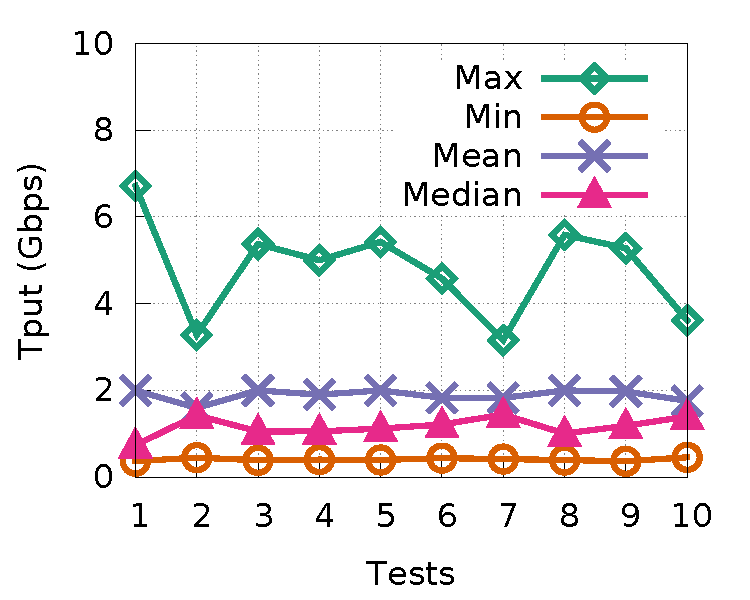
\includegraphics[width=\textwidth]{acdctcp/figures/tput_fairness/default_5CC_tput.pdf}
                %5 CCs
		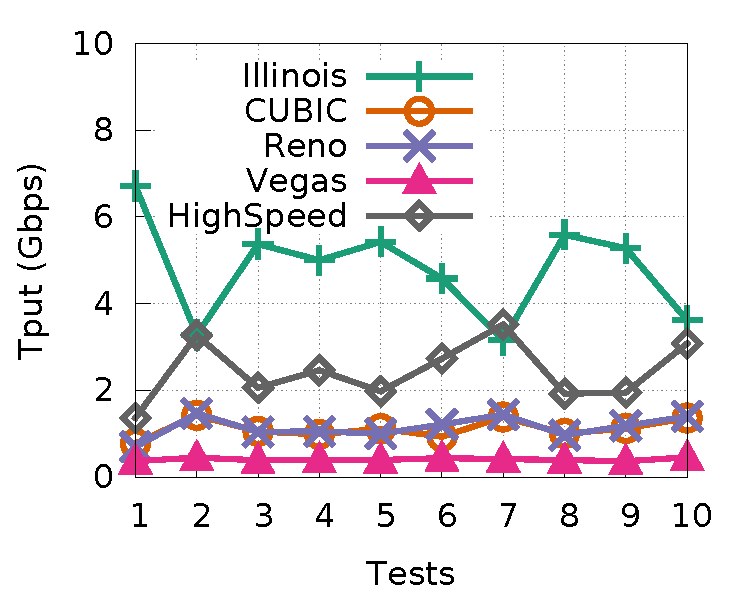
\includegraphics[width=\textwidth]{acdctcp/figures/tput_fairness/default_5CC_tput_detail.pdf}
		\caption{5 different CCs.}
                \label{unfairness_5CC}
        \end{subfigure}
        \begin{subfigure}[b]{0.45\textwidth}
                \centering
                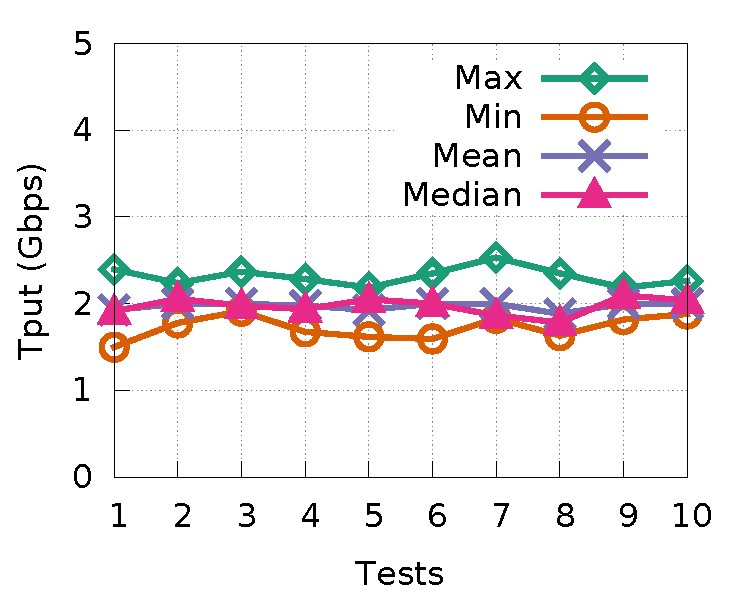
\includegraphics[width=\textwidth]{acdctcp/figures/tput_fairness/default_all_cubic_tput.pdf}
                \caption{All CUBIC.}
                \label{unfairness_all_cubic}
        \end{subfigure}
%        \begin{subfigure}[b]{0.24\textwidth}
%                \centering
%                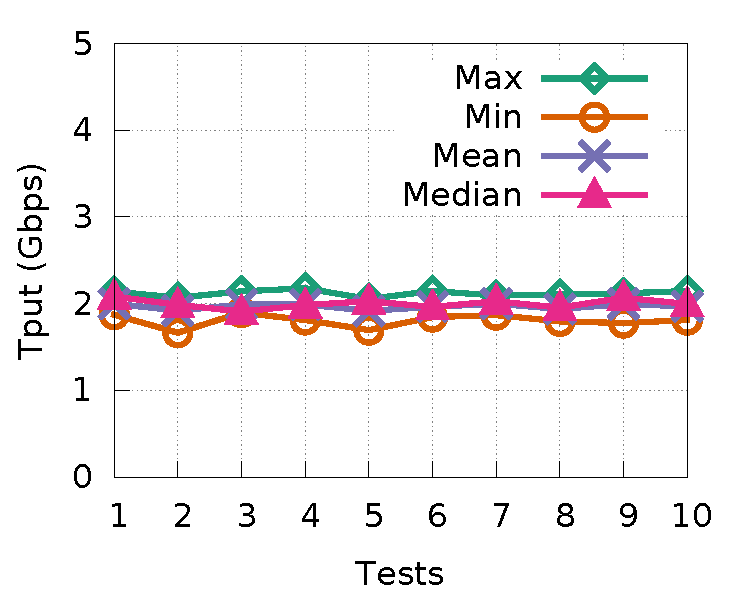
\includegraphics[width=\textwidth]{acdctcp/figures/tput_fairness/liquid_5CC_tput.pdf}
%                \caption{5 different CCs with \acdc{}.}
%                \label{fairness_5CC_with_ours}
%        \end{subfigure}
%        \begin{subfigure}[b]{0.24\textwidth}
%                \centering
%                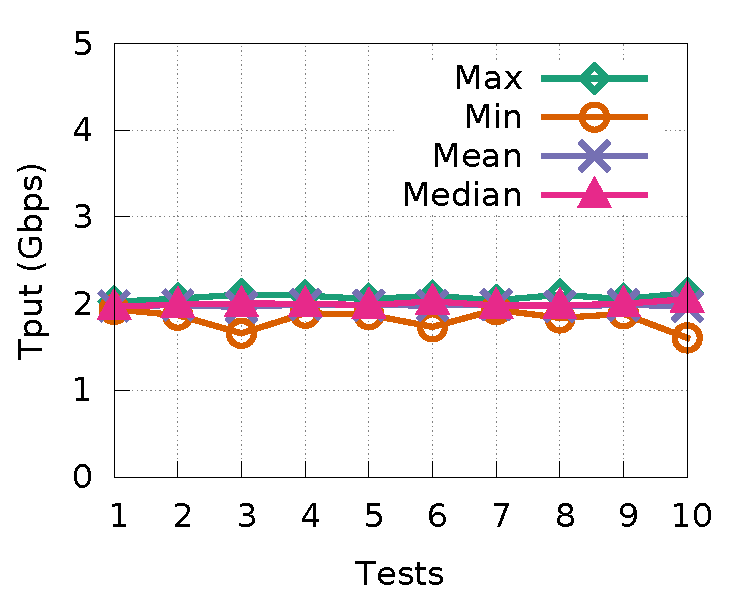
\includegraphics[width=\textwidth]{acdctcp/figures/tput_fairness/ecn_all_dctcp_tput.pdf}
%                \caption{All DCTCP.}
%                \label{fairness_5CC_with_dctcp}
%        \end{subfigure}
        \caption{Different congestion controls lead to unfairness.}
        \label{tput_unfair}
\end{figure}

The next benefit is~\acdc{} allows for {\em uniform}
congestion control to be implemented throughout the datacenter.
Unfairness arises when stacks are handled differently in the fabric or when conservative and aggressive
stacks coexist. Studies have shown ECN-capable and ECN-incapable flows do not exist gracefully on the
same fabric because packets belonging to ECN-incapable flows encounter severe packet drops when their packets
exceed queue thresholds~\cite{wu2012tuning,judd2015nsdi}. %Ideally, tenants shouldn't suffer based on such a simple configuration issue.
%~\eric{Do we have an argument that clients should be able to port their VMs to the cloud without making any changes
%or worrying about the low-level network details of the cloud provider?}
Additionally, stacks with different congestion control algorithms may not share the same fabric fairly.
For example, Figure~\ref{tput_unfair} shows the performance of five different TCP flows on the topology in
Figure~\ref{dumbbell_topology}. Each flow selects a congestion control algorithm available in Linux:
CUBIC~\cite{ha2008cubic}, Illinois~\cite{liu2008tcp}, HighSpeed~\cite{RFC3649},
New Reno~\cite{RFC3782} and Vegas~\cite{Brakmo1994}.
Figure~\ref{unfairness_5CC} shows aggressive stacks such as Illinois and HighSpeed
achieve higher bandwidth and thus fairness is worse than all flows using the
same stack (Figure~\ref{unfairness_all_cubic}). 
%A tenant should not be able
%to unfairly obtain higher bandwidth by simply changing its congestion control.

Another benefit of~\acdc{} is it allows for different congestion control algorithms to be assigned on
a per-flow basis. %Today, TCP congestion control is configured at an OS-level, so all of an OS's flows are forced to use the same congestion control algorithm.
A vSwitch-based approach can assign WAN flows to a congestion control algorithm that optimizes WAN performance~\cite{tan2006compound,flach2013reducing} and
datacenter flows to one that optimizes datacenter performance, even if these flows originate from the same VM (\eg{}a webserver).
%This severely limits flexibility and forces tenants to optimize the performance of a subset of its flows. For example, a web server may choose a TCP stack to optimize
%WAN performance~\cite{tan2006compound,flach2013reducing} at the cost of harming back-end performance within the datacenter.~\eric{still need to clean}
Additionally, as shown in \sref{ss:cc-qos}, a flexible congestion control algorithm can provide relative bandwidth allocations to flows.
This is useful when tenants or administrators want to prioritize flows assigned to the same quality-of-service class.
In short, adjusting congestion control algorithms on a per-flow basis allows for 
enhanced flexibility and performance.
%As studies have shown that TCP can be optimized for datacenters~\cite{dctcp, stephens2014practical, wu2010ictcp,
%mittal2015timely, jose2015high}, WAN environments~\keqiang{cite Compound TCP?}, and even
%~\eric{one more example, wireless/60Ghz/free-space optics?}, selecting a per-flow TCP stack has the potential to
%enhance network performance. By moving congestion control to the vSwitch, administrators can assign a specific congestion control
%algorithm to each flow, optimizing the network performance of its clients in a seamless manner.~\eric{Also add QoS-based CC
%stuff here, since we have something.}

Finally, congestion control is not difficult to port. While the entire TCP stack may seem complicated and prone to high overhead,
the congestion control aspect of TCP is relatively light-weight and simple to implement. Indeed, studies
show most TCP overhead comes from buffer management~\cite{optimize-tcp-receive}, and
in our evaluation the computational overhead of~\acdc{} is less than one percentage point.
Porting is also made easy because congestion control implementations in Linux
are modular: DCTCP's congestion control resides in {\tt tcp\_dctcp.c} and is only about 350 lines of code. Given
the simplicity of congestion control, it is not hard to move its functionality to another
layer.
%~\crs{Furthermore,~\acdc{} does not rate limit or buffer packets, and our
%benchmarks show the computational overhead of~\acdc{} is less than one percentage point.}


\subsection{Tenant-Level Bandwidth Allocation}
%In addition to controlling congestion, public cloud administrators have to find ways to
%isolate the performance of different tenants and applications. 
\crs{While~\acdc{} enforces congestion control, transport layer schemes do not
provide fair bandwidth allocation among tenants because
a tenant with more concurrent flows can obtain
a higher share of bandwidth.
%The situation is further worsened by UDP flows since they are not subjected to any transport
%level congestion control.
In order to provide performance isolation in the network, datacenter operators can implement
a variety of bandwidth allocation schemes by either guaranteeing or proportionally
allocating bandwidth for tenants~\cite{rodrigues2011gatekeeper,Ballani2011oktopus,jeyakumar2013eyeq,shieh2011sharing,
Guo2010Secondnet,Popa2012Faircloud,Xie2012Proteus,Lam2012NetShare,jang2015silo}. 
%Simple static rate limiters enforced on many default public cloud images dictate an upper-bound on the bandwidth available
%to different classes of VMs.
% Congestion can occur when the cumulative bandwidth from a set of
%senders exceeds the bandwidth of a network link (incast is a special case). Consider the topology in Figure~\ref{dumbbell_topology},  
%with 5 flows traversing a bottleneck 10 Gbps link. Even in the case of a "perfect" allocation, where each flow is statically limited to 10 Gbps/5 flows = 2 Gbps,
%the latency caused by queueing heavily depends on the deployed TCP stack. We show this in Figure~\eric{cubic-fill}.
%CUBIC~\cite{ha2008cubic}, the default TCP congestion control algorithm in Linux, will aggressively fill
%the buffer of the congested output port, causing latencies to significantly increase. DCTCP, however, is able
%to keep buffers low~\cite{dctcp}, allowing for a queueing latency that is an order of magnitude lower than CUBIC's. These differences exist despite the fact
%that each scheme is able to achieve the same throughput over the congested link (Section~\ref{results}~\eric{Table 1}).
%Note that in Figure~\ref{cubic-fill}, DCTCP is run in the absence of a static rate limiter, meaning that it is effective
%in mitigating congestion's impact on latency. 
Some of these schemes share high-level architectural similarities to~\acdc{}.}
For example, EyeQ~\cite{jeyakumar2013eyeq} 
%provides a single dedicated switch abstraction for tenant VMs and 
handles bandwidth allocation at
the edge with a work-conserving distributed bandwidth arbitration scheme. It enforces
rate limits at senders based on feedback generated by receivers. Similarly, Seawall~\cite{shieh2011sharing}
provides proportional bandwidth allocation to a VM or application by forcing all
traffic through a congestion-controlled tunnel configured through weights and endpoint feedback.


The fundamental difference between these schemes and our approach is the design
goals determine the granularity on which they operate. 
Performance isolation schemes generally focus on {\em bandwidth allocation on a VM-level} and
are not sufficient to relieve the network of congestion because they do not
operate on flow-level granularity. 
For example, the single switch abstraction
in EyeQ~\cite{jeyakumar2013eyeq} and Gatekeeper~\cite{rodrigues2011gatekeeper} explicitly assumes a congestion-free 
fabric for optimal bandwidth allocation between pairs of VMs. This abstraction doesn't hold in multi-pathed
topologies when failure, traffic patterns or ECMP hash collisions~\cite{hedera} cause congestion in the core.
Communication between a pair of VMs may consist of
multiple flows, each of which may traverse a distinct path. Therefore,
enforcing rate limits on a VM-to-VM level is too coarse-grained to determine how specific flows should adapt in
order to mitigate the impact of congestion on their paths. Furthermore, a scheme like Seawall~\cite{shieh2011sharing}
cannot be easily applied to flow-level granularity because
its rate limiters are unlikely to scale in the number of flows at high networking speeds~\cite{radhakrishnan2014senic}
and its allocation scheme does not run at fine-grained round-trip
timescales required for effective congestion control. Additionally, Seawall violates our design
principle by requiring VM modifications to implement congestion-controlled tunnels.

%Three bandwidth allocation schemes, EyeQ~\cite{jeyakumar2013eyeq}, Gatekeeper~\cite{rodrigues2011gatekeeper} and Seawall~\cite{shieh2011sharing}
%use congestion control techniques to provide bandwidth guarentees. At a high-level, these schemes employ
%VM-to-VM tunnels that partition bandwidth at the network edge (EyeQ) or proportionally allocate bandwidth
%over network links (Seawall). In addition, both EyeQ and Seawall are designed to adapt to network congestion
%by analyzing the fraction of packets marked with ECN bits to adjust the rates imposed on the VM-to-VM tunnels. 
%VM-to-VM tunnels are not fine-grained enough to effective mitigate queueing latencies caused by congestion.
%For example, datacenter topologies typically contain multiple paths from a source to a destination. Therefore,
%if a VM has multiple flows to another VM, those flows may take seperate paths (thanks to ECMP). By combining all flows
%over a single logical VM-to-VM tunnel, the proportion of packets experiencing congestion gets muddled. Flows that
%are not experiencing any congestion get their rates reduced unneccesarrily. Flows that are experiencing congestion
%do not reduce their rates fast enough.~\eric{i know this needs work} 

%\eric{Seawall talk mentioned O($10^5$) new tasks per minute. Can we make something more concrete above?}


\begin{figure}[!t]
        \centering
  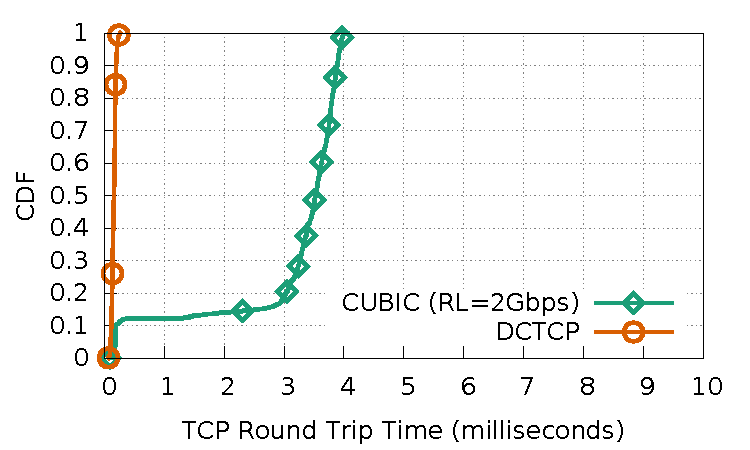
\includegraphics[width=0.7\textwidth]{acdctcp/figures/motivation/motivation_2Gbps_cubic_rl_dctcp_sockperf.pdf}
        \caption{CDF of RTTs showing CUBIC fills buffers.}
        \label{cubic-fill}
\end{figure}
%\subsection{Bandwidth Allocation with Transport Control}
%In fact, bandwidth allocation schemes attempt to provide tenant level performance isolation
%regardless of the tenant transport stack and protocol, even though the stack has a large impact on congestion. 
~\crs{The above points are not intended to criticize any given work, but rather support the argument that
it is important for a cloud provider to enforce {\em both} congestion control and bandwidth allocation.
Congestion control can ensure low latency and high utilization, and
bandwidth allocation can provide tenant-level fairness.}
Bandwidth allocation schemes alone are insufficient to mitigate congestion because certain TCP stacks aggressively
fill switch buffers. Consider a simple example where five flows send simultaneously
on the 10 Gbps topology in Figure~\ref{dumbbell_topology}. Even when the bandwidth is allocated "perfectly"
at 2 Gbps per flow, CUBIC saturates the output port's buffer and leads to inflated round-trip times (RTTs) for traffic
sharing the same link.
%~\footnote{Note the servers are not over-subscribed in this scenario, so even
%bounding rate limiters to 10 Gbps may be deemed satisfactory by some edge-based bandwidth allocation schemes.}. 
Figure~\ref{cubic-fill} shows these RTTs for CUBIC and also DCTCP, 
which is able to keep queueing latencies, and thus RTTs, low even though no rate limiting was applied.
Therefore, it is important for cloud providers to exercise a desired congestion
control.

In summary, our vision regards enforcing tenant congestion control and bandwidth allocation as {\em complimentary} and we claim 
an administrator should be able to
combine any congestion control (\eg{}DCTCP) with any bandwidth allocation scheme (\eg{}EyeQ). 
Flow-level congestion control and tenant performance isolation need not be solved by the same scheme,
so~\acdc{}'s design goal is to be modular in nature so it can co-exist with any bandwidth allocation scheme
and its associated rate limiter (and also in the absence of both). 
%To the best of our knowledge,~\acdc{} is the first work that advocates moving flow-level transport congestion control
%out of the VM and into the hypervisor.~\eric{keep?}

%~\eric{is this fair in respect to seawall? and what about NICs that support full TCP offload?}
%A key design goal of~\acdc{} is for it to be modular in nature so it can co-exist with any bandwidth allocation scheme 
%and its associated rate-limiter (and also in the absence of both).
%In order to achieve this goal,~\acdc{} satisfies a variety of constraints. First, it is
%computationally light-weight in order to minimize the overhead of its adoption. Second,
%it doesn't require any changes to VMs or network hardware so it can be deployed in
%current and future networks. Third, our scheme works in the absence of specific topology
%information and works over arbitrary topologies. Fourth, it does not require
%any information about tenant traffic patterns or require specific VM placement or admission
%mechanisms.
%
